% LaTeX Template for Project Report, Version 1.0
% (Abstracted for a Value Education Project Report at NIT Calicut but can be
% modified easily to use for other reports also.)
%
% Released under Creative Commons Attribution license (CC-BY)
%
% Created by: Kartik Singhal
% BTech CSE Batch of 2009-13
% NIT Calicut
% Contact Info: kartiksinghal@gmail.com
%
% It is advisable to learn the basics of LaTeX before using this template.
% A good resource to start with is http://en.wikibooks.org/wiki/LaTeX/
%
% All template fields are marked with a pair of angular brackets e.g. <title here>
% except for the ones defining citation names in ref.tex.
%
% Empty space after chapter/section/subsection titles can be used to insert text.
%
% Just compile this file using pdflatex after making all required changes.

\documentclass[12pt,a4paper]{report}
\usepackage[pdftex]{graphicx} %for embedding images
\usepackage{url} %for proper url entries
\usepackage[bookmarks, colorlinks=false, pdfborder={0 0 0}, pdftitle={A Food Review App for iPhone}, pdfauthor={Xinjiang Shao}, pdfsubject={UIC Project Report}, pdfkeywords={iOS, Foodie, Social, Location, Review}]{hyperref} %for creating links in the pdf version and other additional pdf attributes, no effect on the printed document
\usepackage[final]{pdfpages} %for embedding another pdf, remove if not required
\usepackage{figsize}

\begin{document}
\renewcommand\bibname{References} %Renames "Bibliography" to "References" on ref page

%include other pages
\begin{titlepage}

\begin{center}

\textup{\large A report on}\\[1.0cm]

% Title
\uppercase{\Large \textbf {Fancy Foodie : A Food Review App for iPhone}}\\[3.0cm]

% Done by
\normalsize Done by \\
\begin{table}[h]
\centering
\begin{tabular}{lr}\hline \\
Full Name & Xinjiang Shao \\ 
UIN & 675469866 \\ \\ \hline
\\
Advisor & Jakob Eriksson \\
Secondary Committee & Ugo Buy \\ \\ \hline 
\end{tabular}
\end{table}

\vfill

% Bottom of the page

\includegraphics[width=0.60\textwidth]{./uic-logo}\\[1cm]
\LARGE{Department of Computer Science}\\
\normalsize
\textsc{University of Illinois at Chicago}\\
%Calicut, Kerala 673 601 \\
\vspace{0.5cm}
Spring 2013

\end{center}

\end{titlepage}

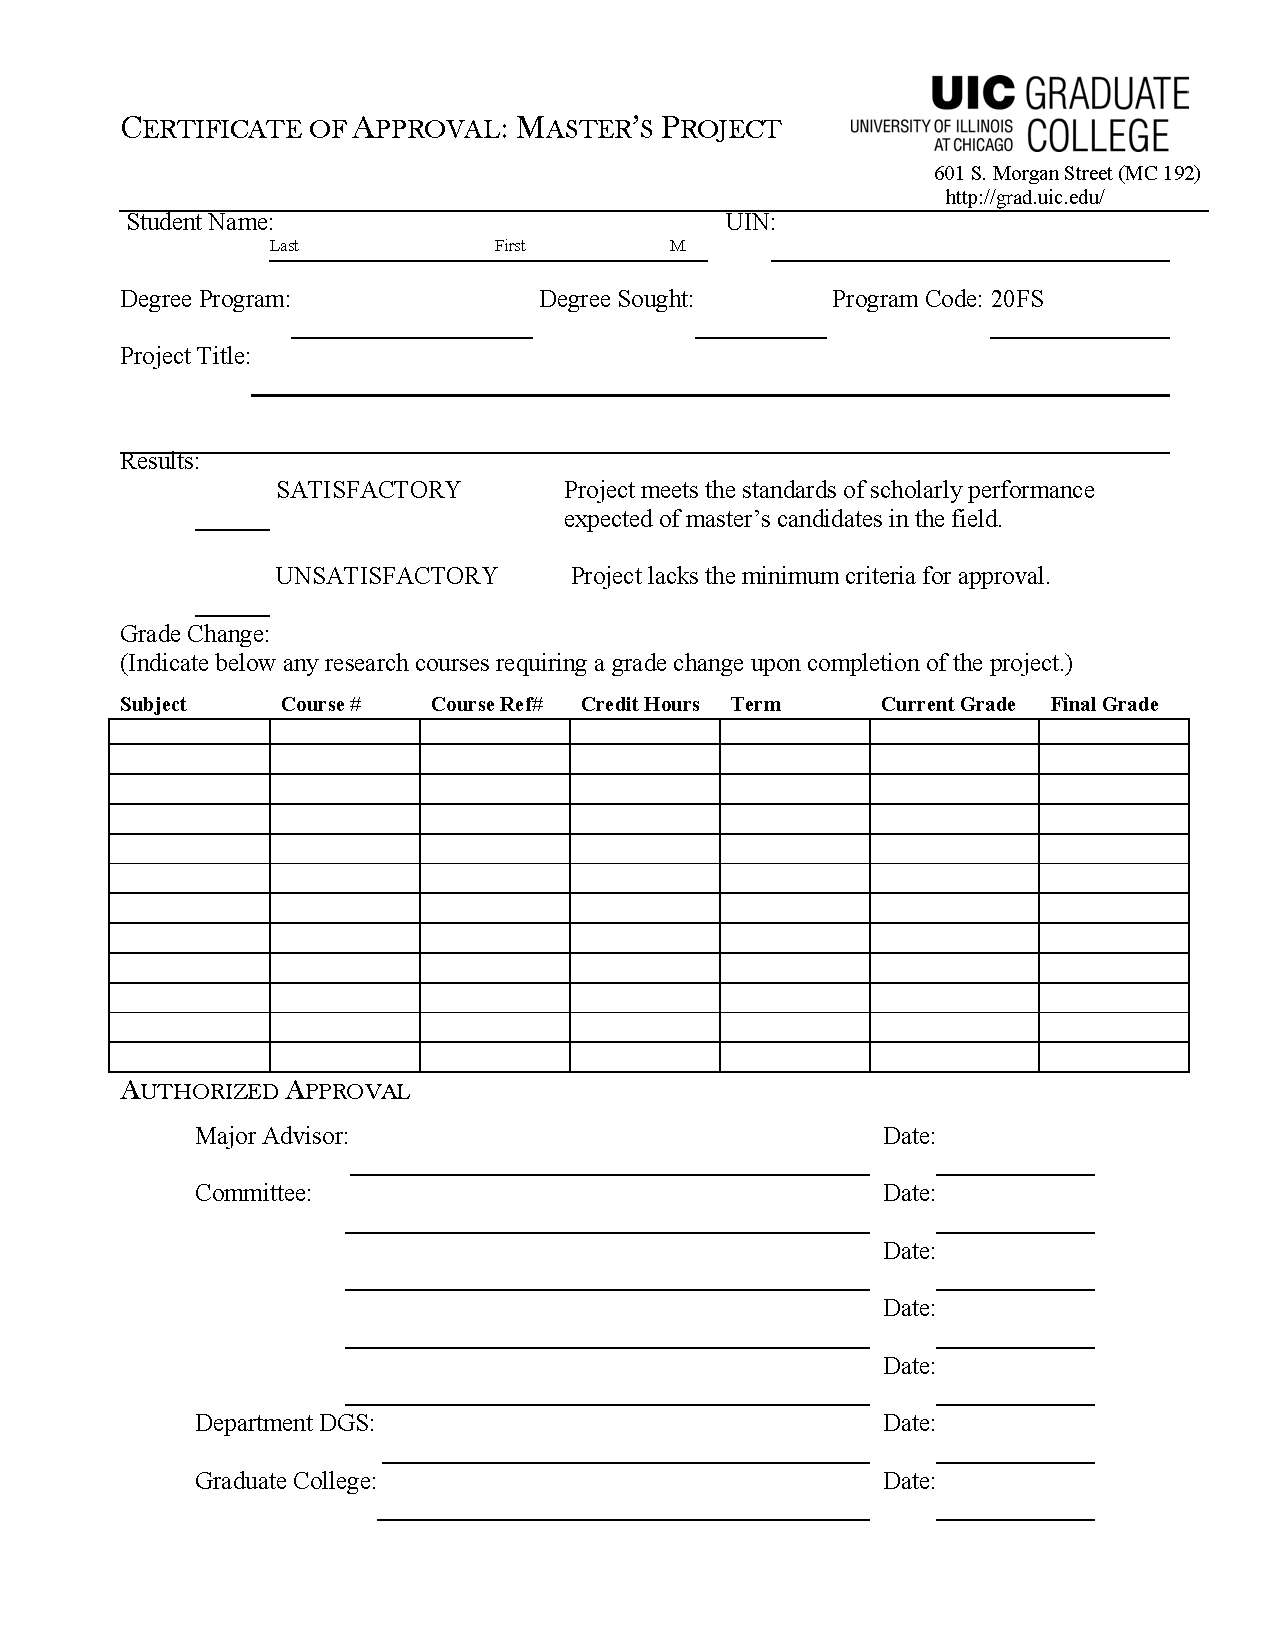
\includepdf{./CertificateofApprovalMAproject.pdf}
\vspace{2in}
\begin{abstract}

Food review is become trendy among young people since smart phone get more and more popular. However, not many tools available for people to review a cuisine and publish their comment to social media conveniently in the market. This project is meant to develop an iOS App called \emph{Fancy Foodie} that can take picture of food, attach meta data such as location, rate, comment, date, tags to the picture and sharing with friends via social media including Facebook, Twitter, Weibo etc.. The App also provides ways to search events by address and review statistic of all events. 

\end{abstract} 


\pagenumbering{roman} %numbering before main content starts
\tableofcontents
\listoffigures

\newpage
\pagenumbering{arabic} %reset numbering to normal for the main content

\chapter{Introduction}

Mobile Apps are making our life more and more interesting than ever before. A lot of young people love to take photo with their smart phone, making comments to it and sharing with their friend about what they had done. I personally find it would be useful if there is a tool for anyone to create food event and share with friends. \\


This project is a food review application called ``Fancy Foodie'' for iOS. The particular aim of the project is to be able to review food and sharing food event with friends. Before you start eating, the user would take a picture of the food they are going to eat and give some basic information about location, tags, date etc. Tags are used to describe the type of the food such as ``Chinese, Bun'' or ``Tea, Classic, Jasmine Green''. After finish eating, the user would make comments of the food. This application also lets user search nearby location or location defined by user, which will show a list of pins on the map where the user had been there before, to decide what the user want to eat. When the user saves a food event, he or she may also share the review and foodie's photo to Facebook or Twitter or to an email address. For user to see the history records, the application also provide a way to view statistics data such as how many places the user has been, how the rates are, how many tags the user used etc. ?\\


Currently, various of apps related to foodie are available in apple's app store. But most of them focused on the whole store/restaurant review. This could be inaccurate sometimes because you might just hate one dish. And there are also a few recipe-related apps. But the project want to have a better tool to publish what you eat instead of how that dish is made. \\ 


\chapter{The Graphic User Interface} % (fold)
\label{cha:the_graphic_user_interface}

\section{Home Tab} % (fold)
\label{sec:tabs}
	As shown in Figure~\ref{fig:hometab}, home tab is created for adding new event to the app. The default view for user when entering the app is the view shown in Figure~\ref{fig:guideview}. \\
	
	Figure~\ref{fig:guideview} gives a short tutorial for user. If the user chooses the plus sign in navigation bar, another blank view with black background should show up. After tapping on the camera icon in navigation bar, View in Figure~\ref{fig:pickaction} will display an action sheet including ``Use Last Photo Taken'', ``Take Photo'', ``Choose from Library'' and ``Cancel''. Here we use ``Take Photo'' as an example. For instance, we choose ``Take Photo'', the app should pop up a modal and let user take picture of food. A modal like Figure~\ref{fig:moveandscale} should appear for user to move and scale the photo to a right position and size after choosing a picture. Figure~\ref{fig:didpick} will show up after scaling step. If no photo is chosen, a warning will show up which alerts user to add a photo first. Tapping on next to move to next view as shown in Figure~\ref{fig:moreinfo}. In this view, a form is created for user to fill in location information, date, tags, comment and rate. Since the user just starts to eat, comment and 
rate field can be empty for now. Other fields should be filled correctly in this view because the user won't be able to edit all the other fields once saved the event. In Figure~\ref{fig:locationpicker}, the location list is generated through Foursquare Application Programming Interface(API). Foursquare API is chosen  because it has a good reputation in both academic and industry world for rich venues in their database. By passing current longitude and latitude, we're able to have a venue list based the distance.

\begin{figure}
    \centering
    \SetFigLayout{3}{3}
    \subfigure[Guide View]{
	\label{fig:guideview}
	
\includegraphics[width=\figwidth, totalheight=\figheight, keepaspectratio]{./screenshots/home.png}} \hfill
    \subfigure[Pick Action]{
	\label{fig:pickaction}
	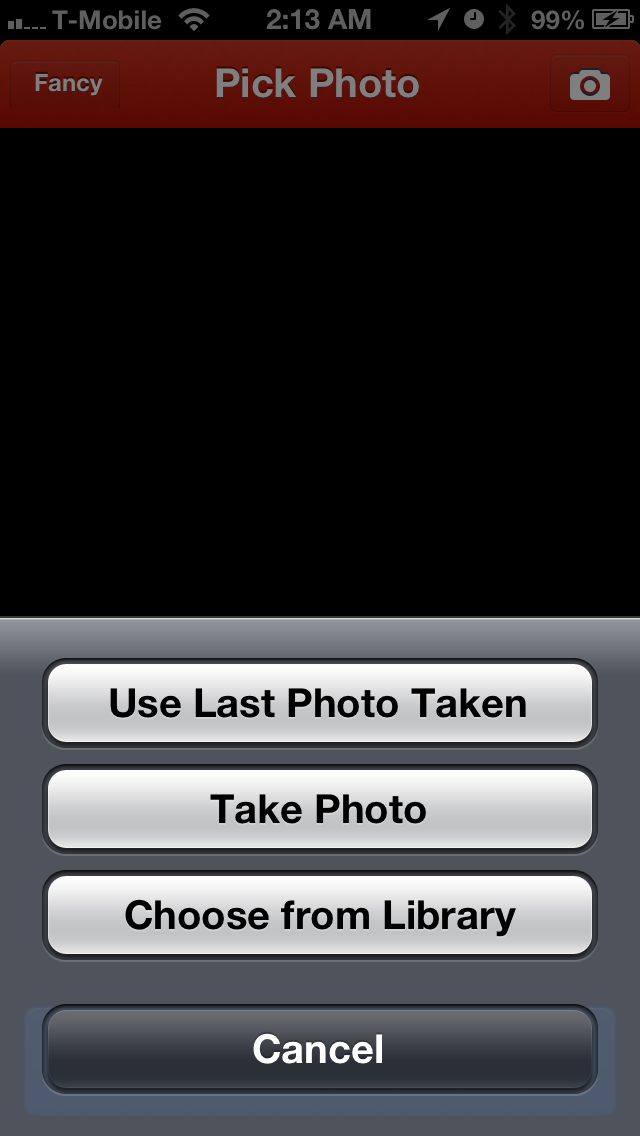
\includegraphics[width=\figwidth, totalheight=\figheight, keepaspectratio]{./screenshots/home-pickaction.png}} \hfill
	\subfigure[Move and Scale]{
	\label{fig:moveandscale}
	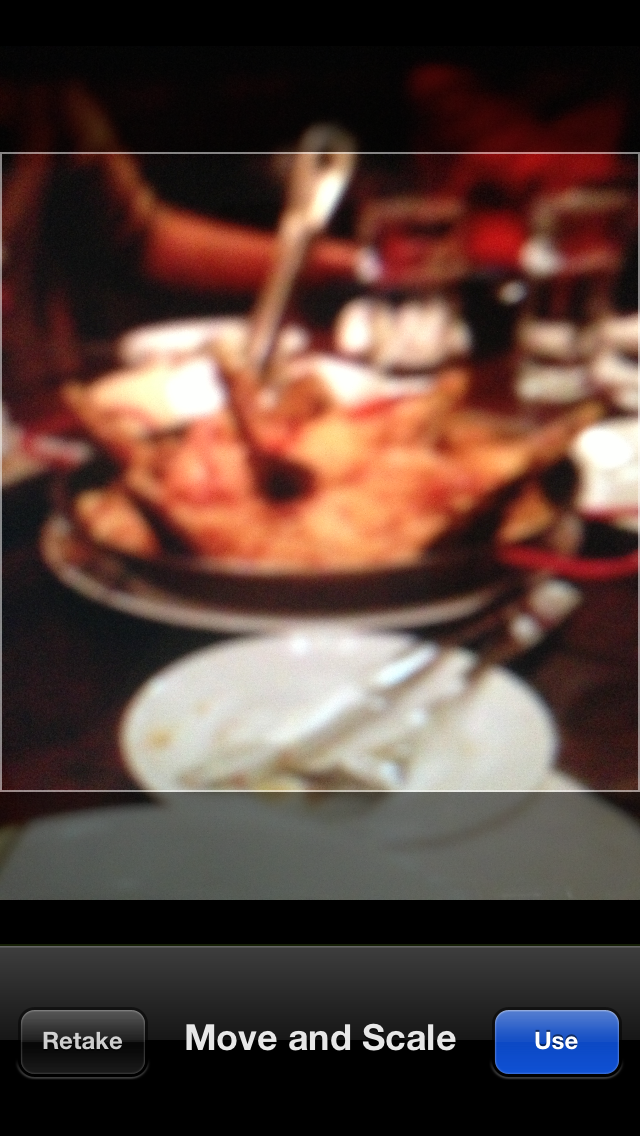
\includegraphics[width=\figwidth, totalheight=\figheight, keepaspectratio]{./screenshots/home-moveandscale.png}} \hfill \\
    \subfigure[After Picking]{
	\label{fig:didpick}
	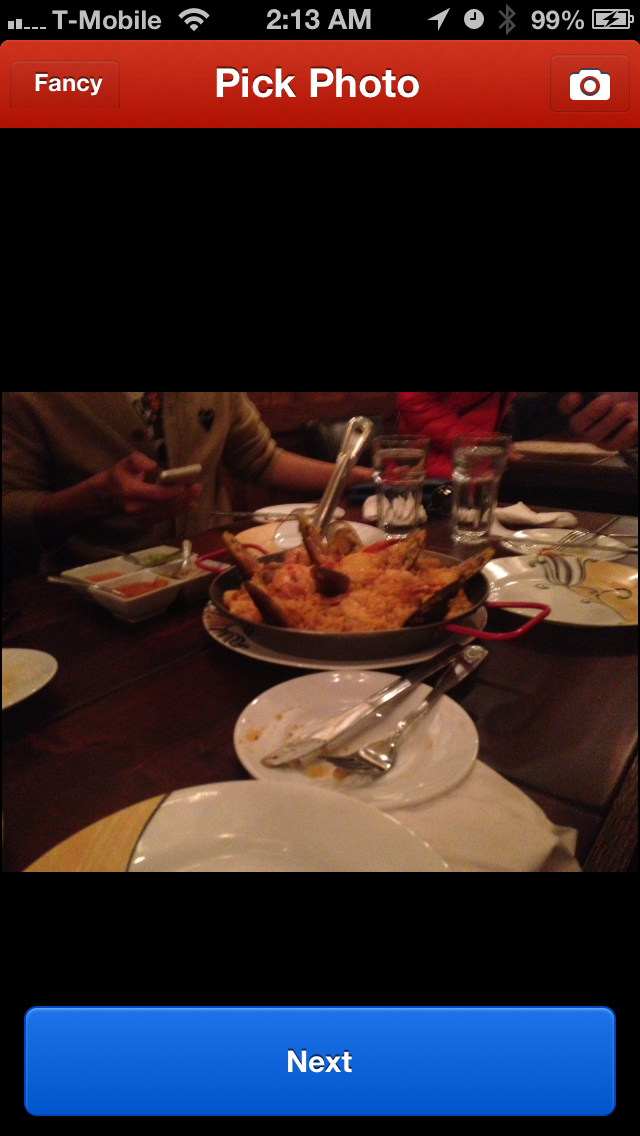
\includegraphics[width=\figwidth, totalheight=\figheight, keepaspectratio]{./screenshots/home-didpick.png}} \hfill
	\subfigure[Event Form]{
	\label{fig:moreinfo}
	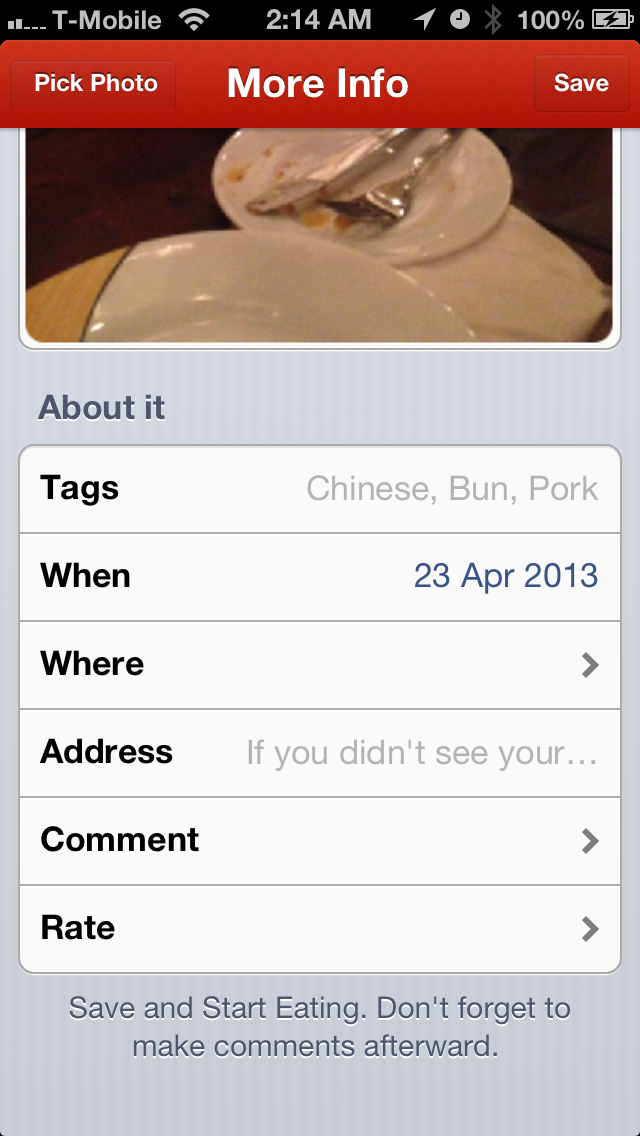
\includegraphics[width=\figwidth, totalheight=\figheight, keepaspectratio]{./screenshots/home-moreinfocontd.png}}   \hfill
    \subfigure[Date Picker]{
	\label{fig:datepicker}
	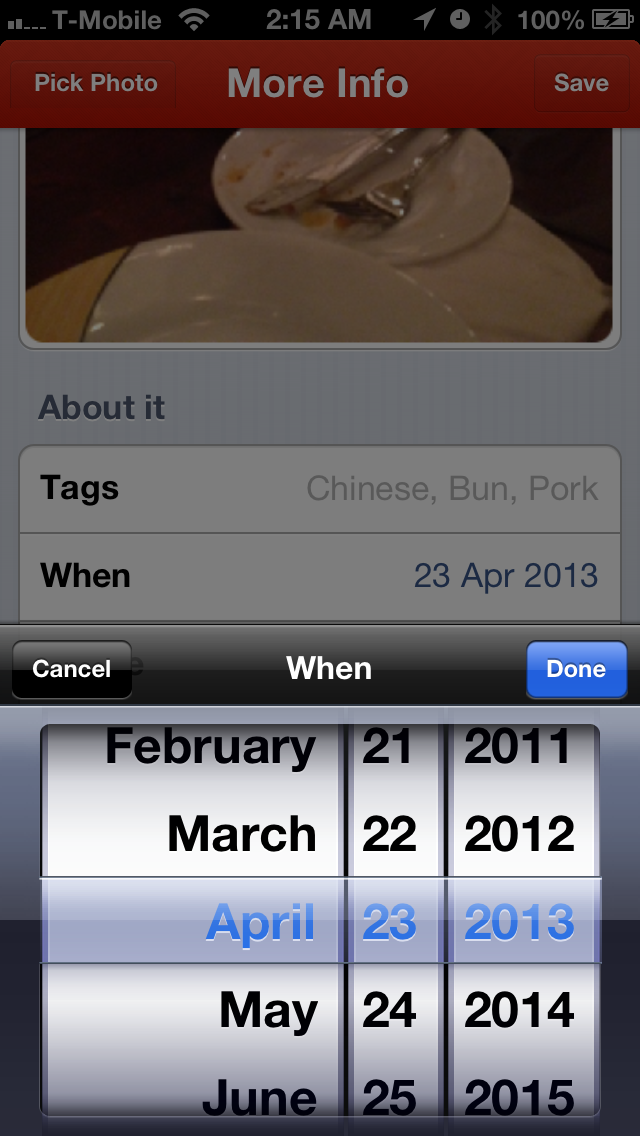
\includegraphics[width=\figwidth, totalheight=\figheight, keepaspectratio]{./screenshots/home-when.png}} \hfill \\
    \subfigure[Location Picker]{
	\label{fig:locationpicker}
	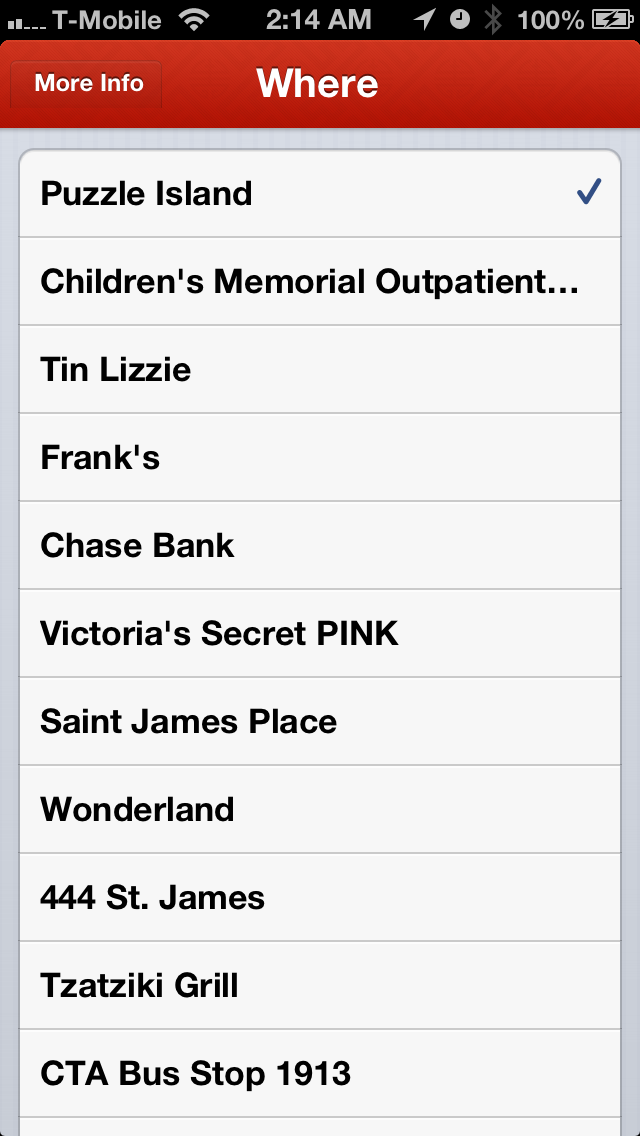
\includegraphics[width=\figwidth, totalheight=\figheight, keepaspectratio]{./screenshots/home-where.png}} \hfill
	\subfigure[Comment Editor]{
	\label{fig:commenteditor}
	
\includegraphics[width=\figwidth, totalheight=\figheight, keepaspectratio]{./screenshots/home-comment.png}}  \hfill
	\subfigure[Rate Picker]{
	\label{fig:ratepicker}
	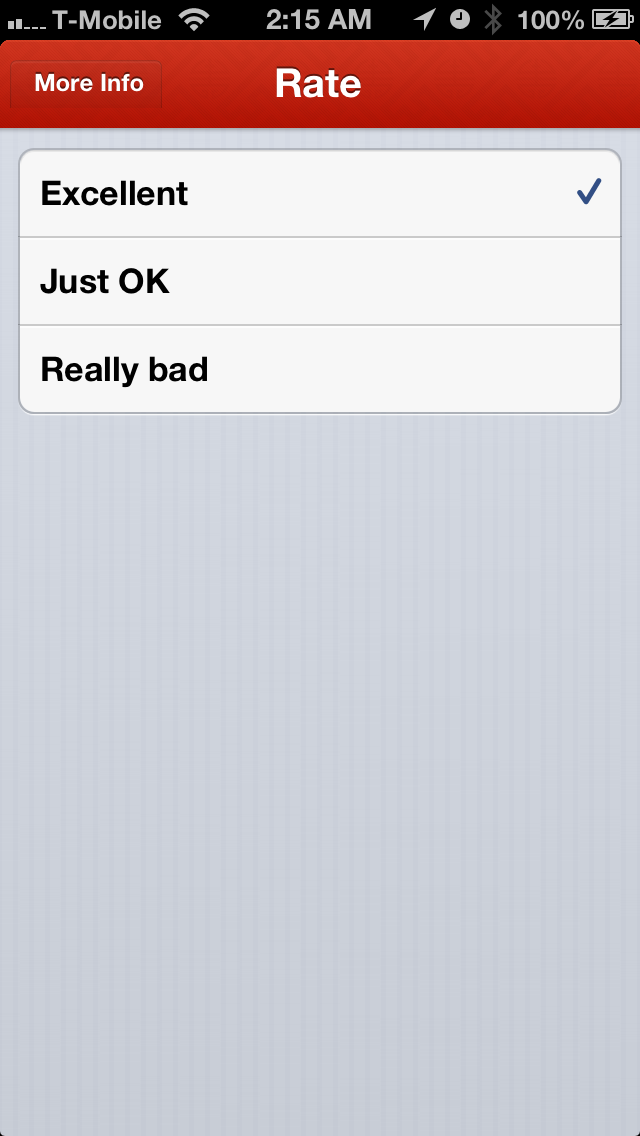
\includegraphics[width=\figwidth, totalheight=\figheight, keepaspectratio]{./screenshots/home-rate.png}} \hfill
	\caption{Home Tab View}
	\label{fig:hometab}
\end{figure}



% section tabs (end)

\section{Food List Tab} % (fold)
\label{sec:foodie_list_tab}

   In food list tab, it fetches a list of food events ordered by creation date. Figure~\ref{fig:foodlist} shows some events. On each table cell, it shows a thumbnail, relative date and event location name. A green menu pop up button is created for sharing with social media(Figure~\ref{fig:foodlist-share}), updating comment(Figure~\ref{fig:foodlist-comment}) and changing rate(Figure~\ref{fig:foodlist-rate}). \\
   
   After choosing one event, a detail view of the event will appear as shown in Figure~\ref{fig:foodlist-detail} and Figure~\ref{fig:foodlist-detailcontd}. You could see all the detailed information here which stored in the local database. In the top navigation bar, a sharing button displays in order to let user publish the event conveniently. If the user chooses Twitter, it'll check if he is logged in Twitter or not. After making sure the user have a Twitter account, Figure~\ref{fig:foodlist-twitter} will appear. The comment and photo is generated by the app. Simply tapping on send, and the event will be shared. \\
   

\begin{figure}
    \centering
    \SetFigLayout{3}{3}
    \subfigure[Food List]{
	\label{fig:foodlist}
	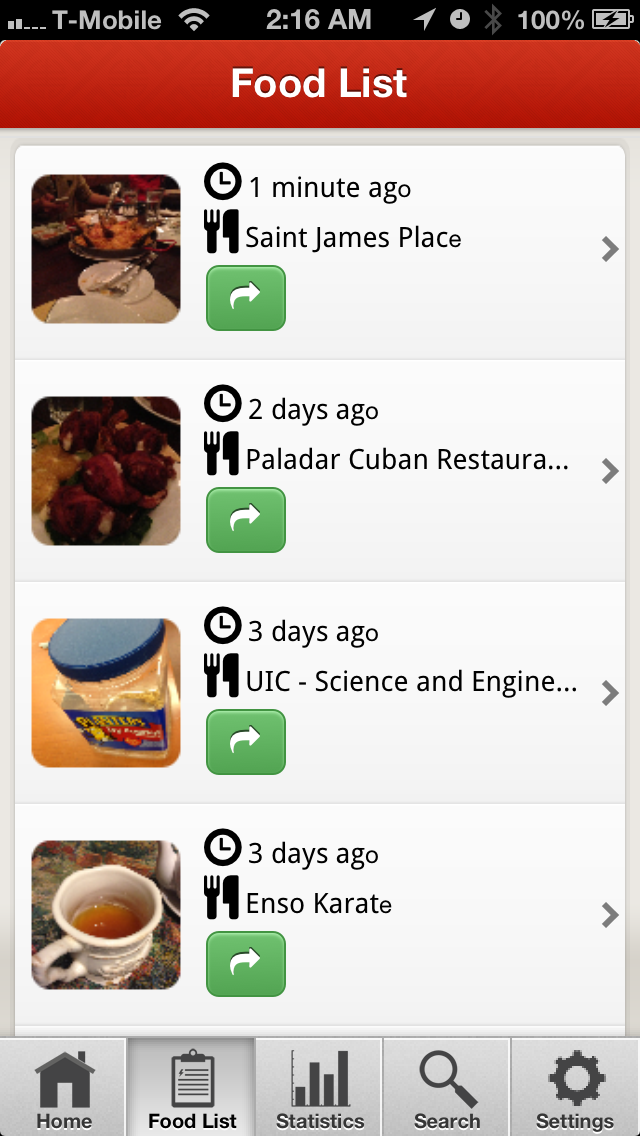
\includegraphics[width=\figwidth, totalheight=\figheight, keepaspectratio]{./screenshots/foodlist.png}} \hfill
	\subfigure[Menu Pop-up]{
	\label{fig:foodlist-menu}
	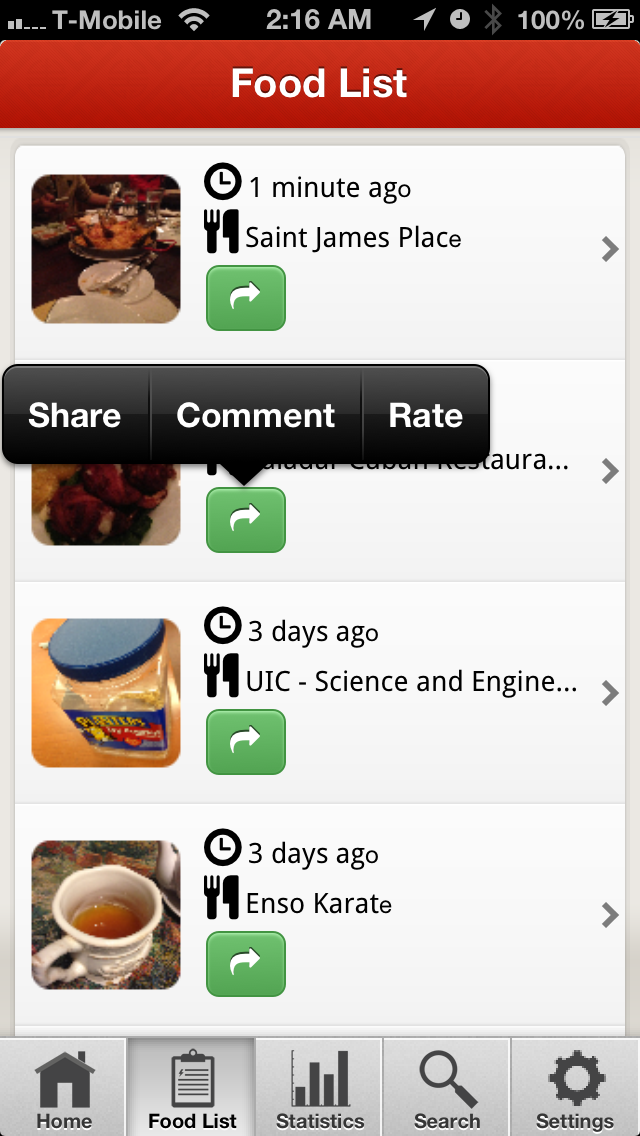
\includegraphics[width=\figwidth, totalheight=\figheight, keepaspectratio]{./screenshots/foodlist-menupop.png}} \hfill 
	\subfigure[Comment Editor]{
	\label{fig:foodlist-comment}
	
\includegraphics[width=\figwidth, totalheight=\figheight, keepaspectratio]{./screenshots/foodlist-comment.png}} \hfill \\
    \subfigure[Rate Action Sheet]{
	\label{fig:foodlist-rate}
	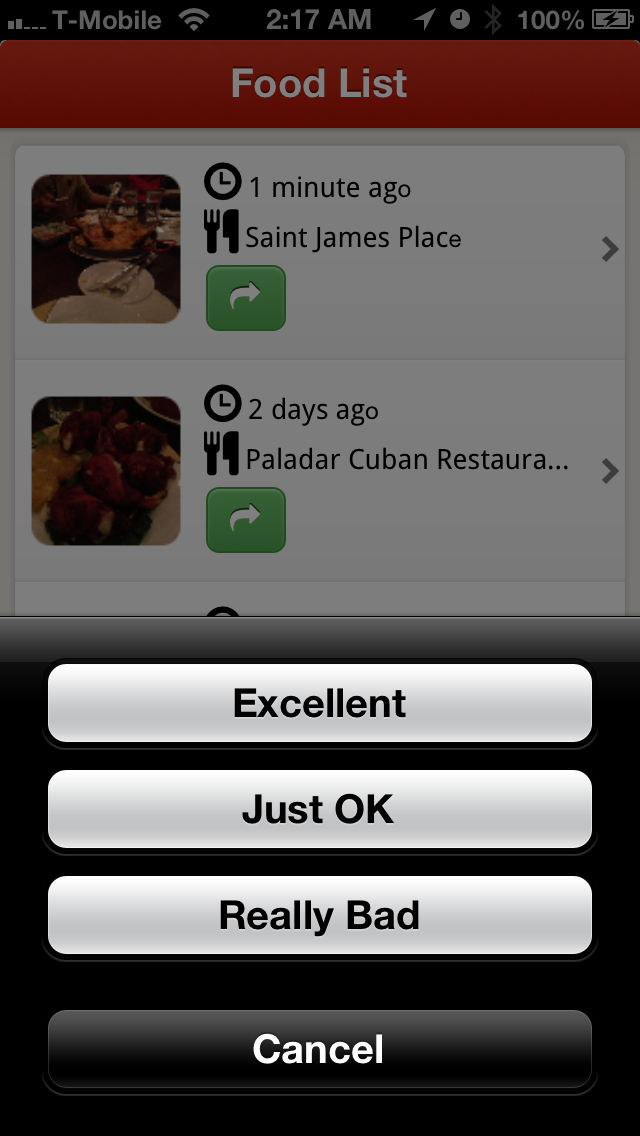
\includegraphics[width=\figwidth, totalheight=\figheight, keepaspectratio]{./screenshots/foodlist-rate.png}} \hfill
	\subfigure[Sharing Activity Controller]{
	\label{fig:foodlist-share}
	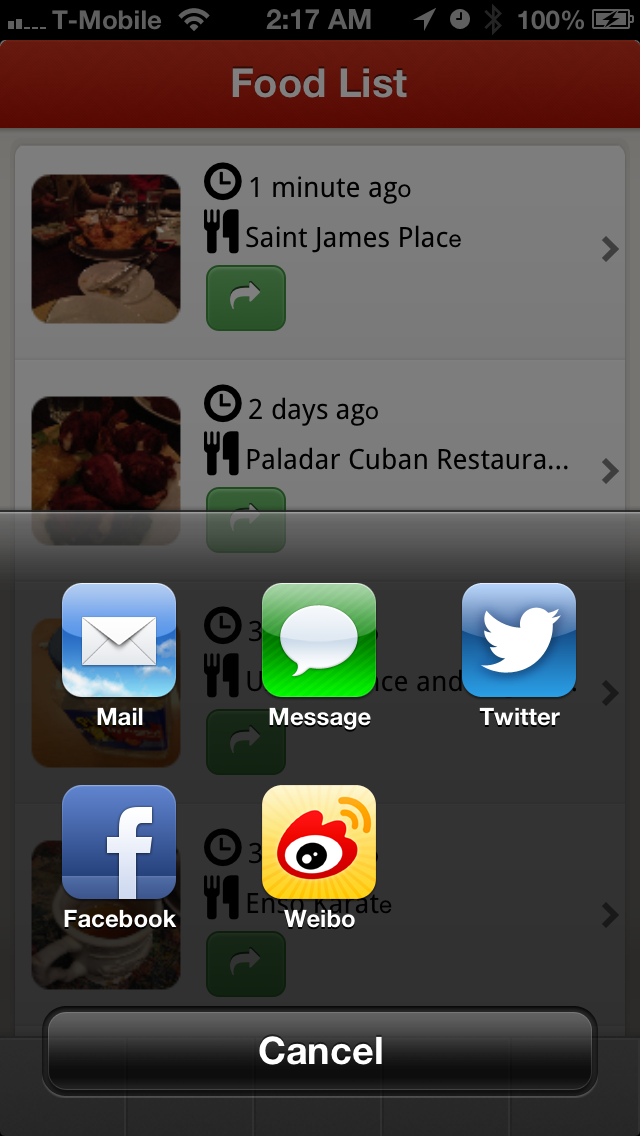
\includegraphics[width=\figwidth, totalheight=\figheight, keepaspectratio]{./screenshots/foodlist-share.png}} \hfill 
	\subfigure[Detail View]{
	\label{fig:foodlist-detail}
	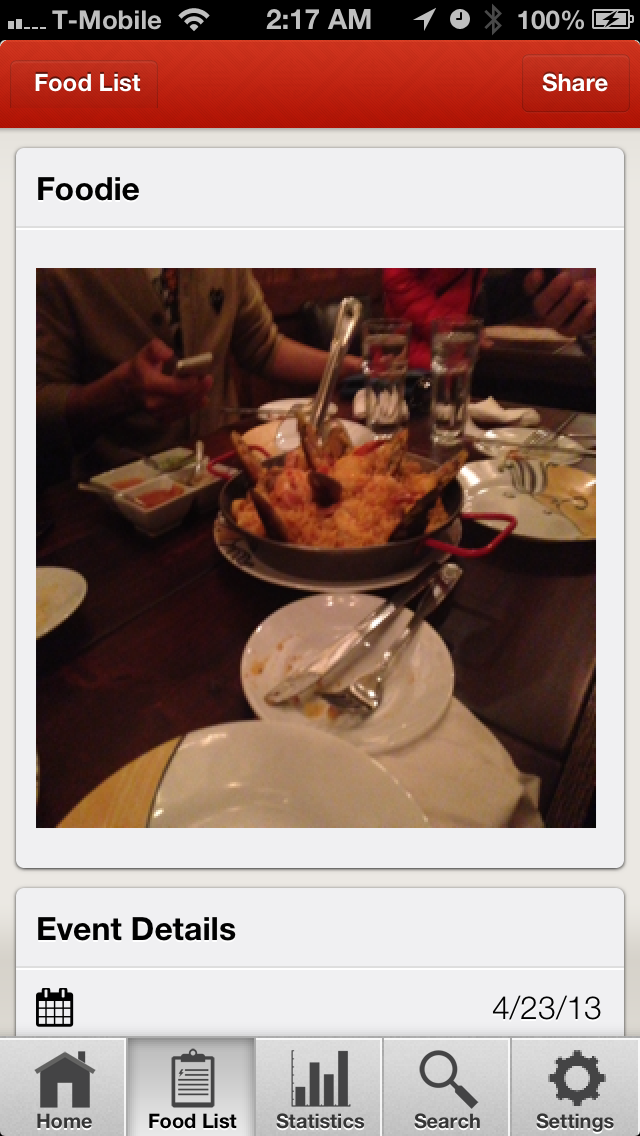
\includegraphics[width=\figwidth, totalheight=\figheight, keepaspectratio]{./screenshots/foodlist-detail.png}} \hfill \\
	\subfigure[Detail View Cont'd]{
	\label{fig:foodlist-detailcontd}
	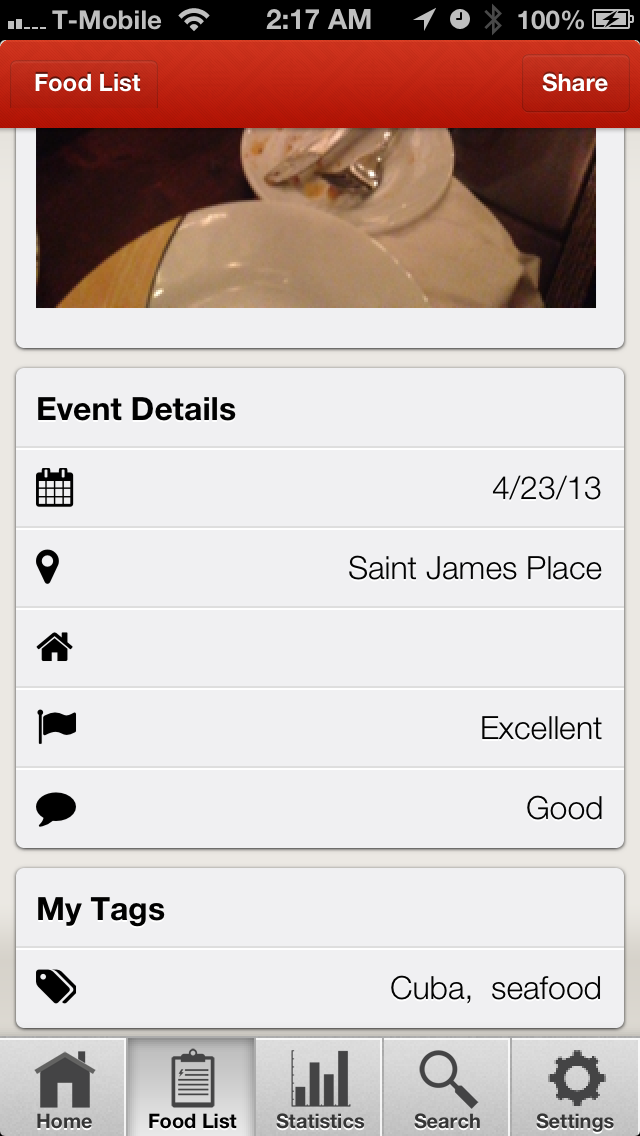
\includegraphics[width=\figwidth, totalheight=\figheight, keepaspectratio]{./screenshots/foodlist-detailcontd.png}} \hfill
	\subfigure[Twitter]{
	\label{fig:foodlist-twitter}
	
\includegraphics[width=\figwidth, totalheight=\figheight, keepaspectratio]{./screenshots/foodlist-twitter.png}} \hfill
	\subfigure[Delete View]{
	\label{fig:foodlist-delete}
	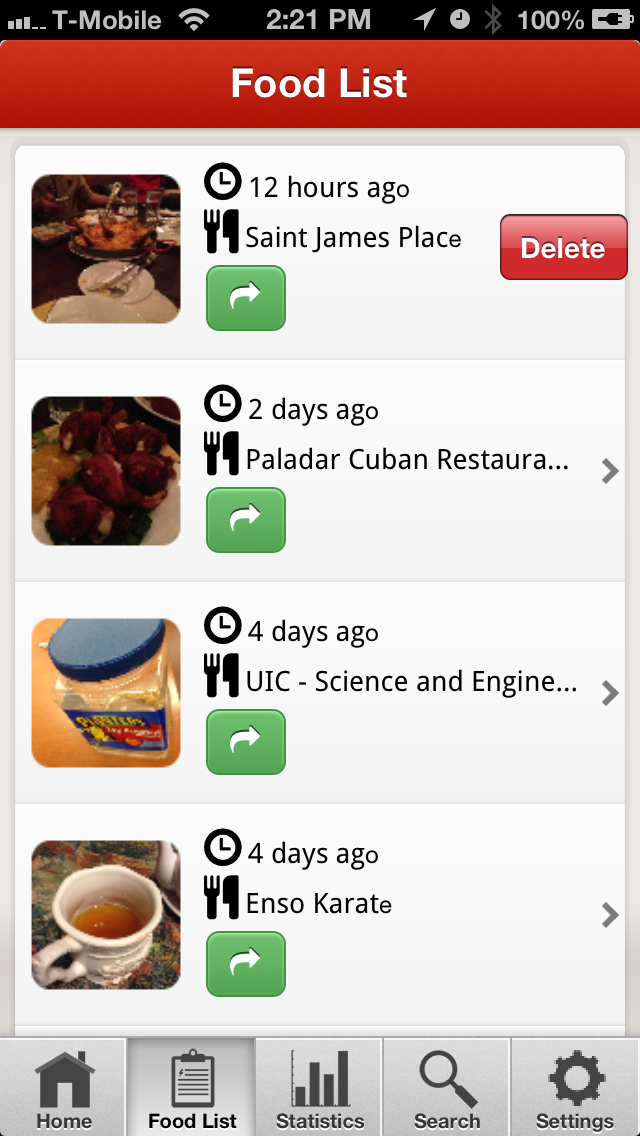
\includegraphics[width=\figwidth, totalheight=\figheight, keepaspectratio]{./screenshots/foodlist-delete.png}} \hfill
	\caption{Food List Tab View}
	\label{fig:foodielisttab}
\end{figure}

% subsection food_list_tab (end)

\section{Statistics Tab} % (fold)
\label{sec:stats_tab}

Statistics tab is supposed to give the user an overview of all events he created. As shown in Figure~\ref{fig:stats}, ``Rates'' are clustered in different categories. All the tags are counted and shown in the table. The total number of places are shown in the table as well. In this way, the user could easily get an idea of what kind of places and food he likes.
  
\begin{figure}
	\centering
    \SetFigLayout{1}{1}
    {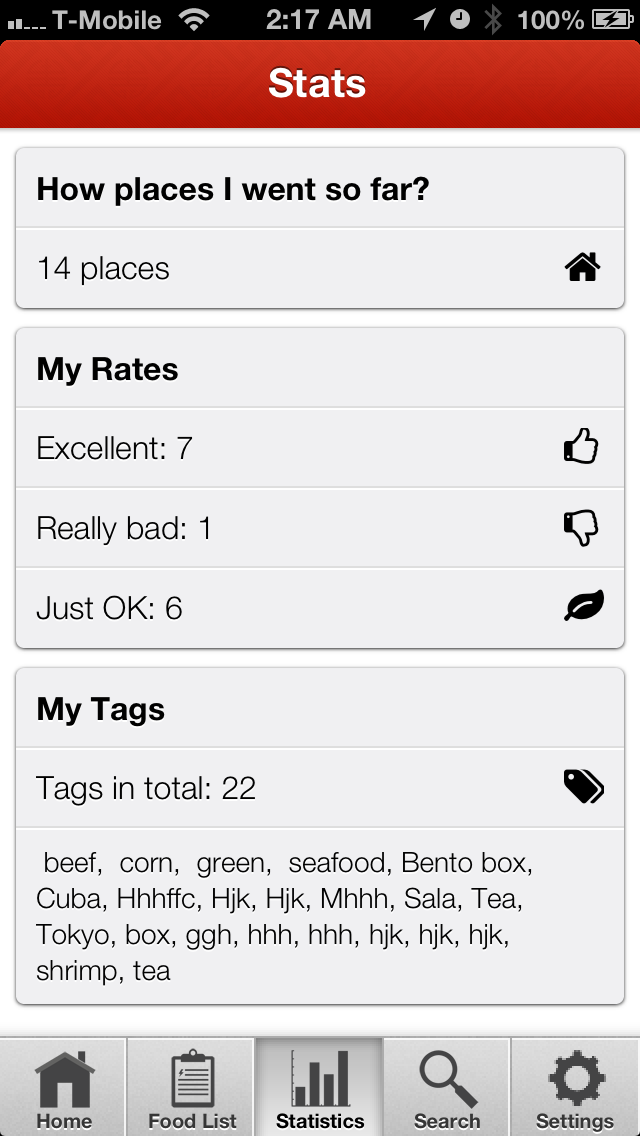
\includegraphics[%
    width=\figwidth, totalheight=\figheight, keepaspectratio]{./screenshots/stats.png}}
    \caption{Statistics Tab View}
	\label{fig:stats}
\end{figure}

% subsection stats_tab (end)
\section{Map Tab} % (fold)
\label{sec:map_tab}

In Figure~\ref{fig:map}, all the event locations are labeled with red pins. By default, it is showing the events around your current location. But you could also change your view by passing address in Figure~\ref{fig:map-address}. After choosing a location in the list, the table view will be dismissed and the new central region will be the location you chose. 

\begin{figure}
	\centering
    \SetFigLayout{1}{2}
	\subfigure[Map]{
	\label{fig:map}
	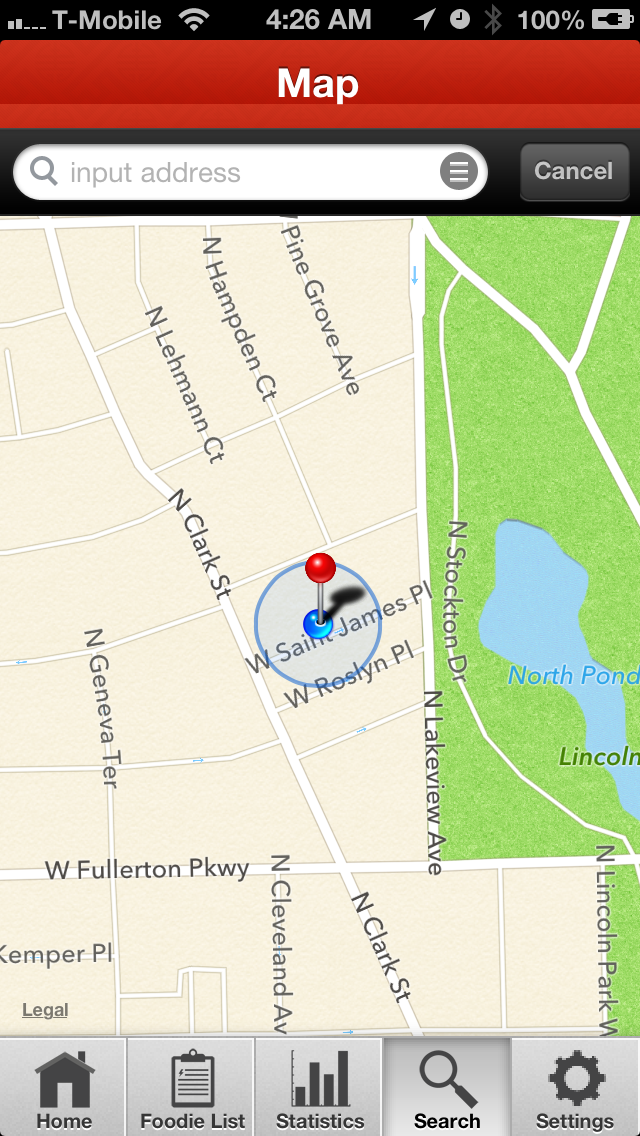
\includegraphics[width=\figwidth, totalheight=\figheight, keepaspectratio]{./screenshots/map.png}} \hfill
	\subfigure[Address Searching]{
	\label{fig:map-address}
	
\includegraphics[width=\figwidth, totalheight=\figheight, keepaspectratio]{./screenshots/map-address.png}} \hfill
    \caption{Map Tab View}
\end{figure}

% subsection map_tab (end)

\section{Setting Tab} % (fold)
\label{sec:setting_tab}

Setting tab provides a view to setup configurations of the app (Figure~\ref{fig:settings}). The view in this tab is a static table view built in storyboard. A web-view controller is created to show the app website and author introduction. By turning on the \emph{save photo} option, it will save the photo to an album. The feedback option is used for user to submit feedback through TestFlight. TestFlight is a online tool to do open beta testing on the fly. By hooking with TestFlight, we will be able to see all the crash reports, time durations for each session, and even ask questions to users when a checkpoint is reached.\\


\begin{figure}
	\centering
    \SetFigLayout{2}{2}
	\subfigure[Settings]{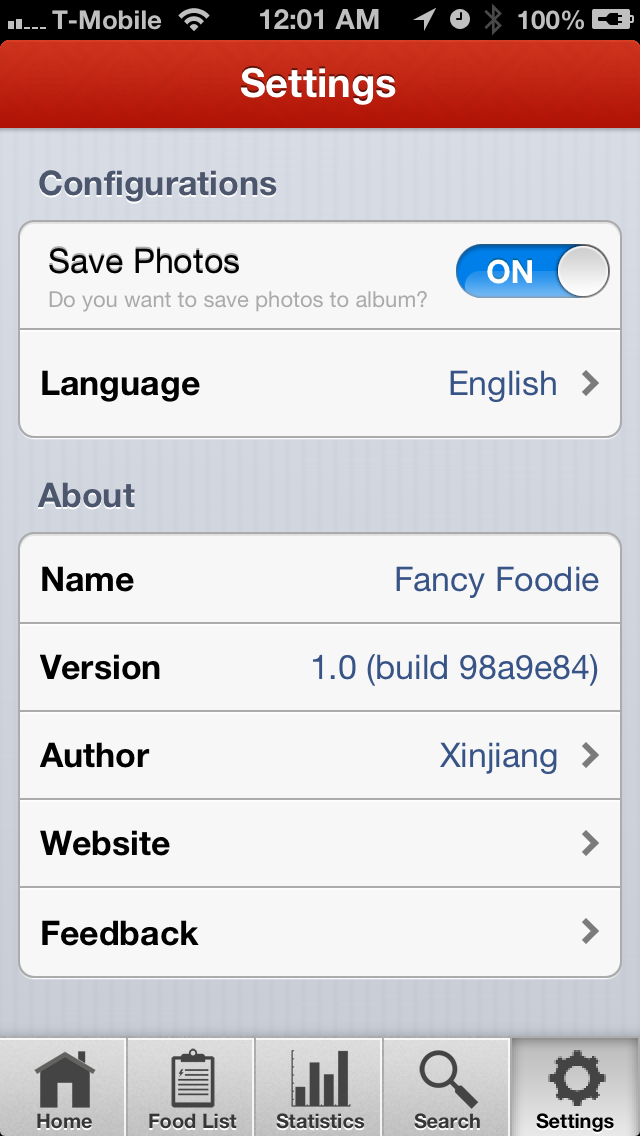
\includegraphics[width=\figwidth, totalheight=\figheight, keepaspectratio]{./screenshots/settings.png}} \hfill
	\subfigure[Save to Album]{
	\label{fig:album}
	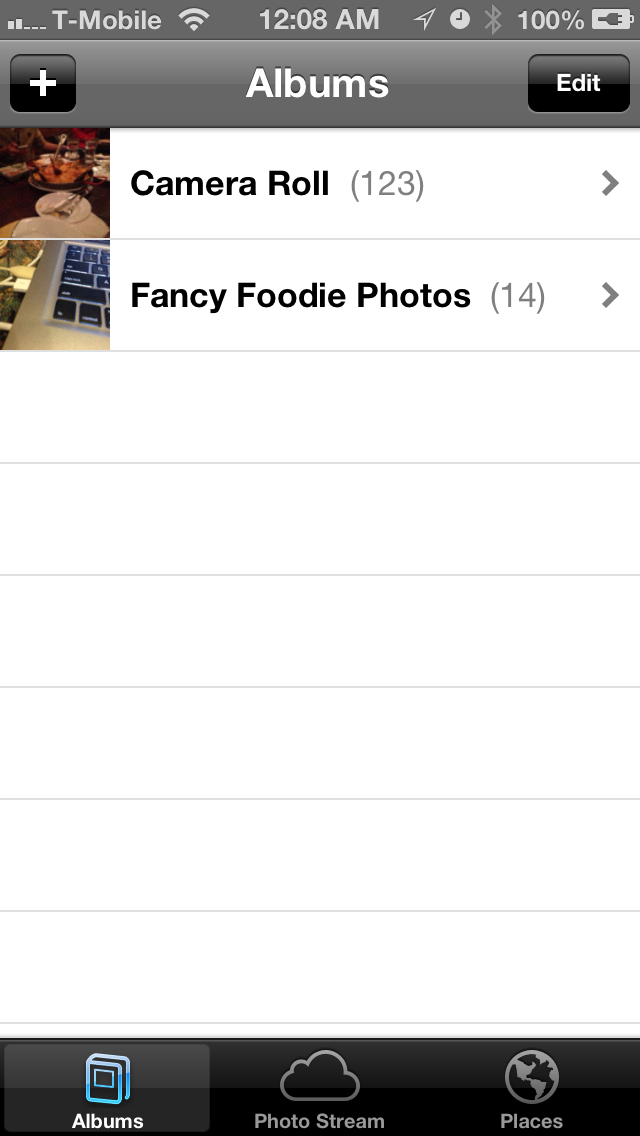
\includegraphics[width=\figwidth, totalheight=\figheight, keepaspectratio]{./screenshots/settings-album.png}} \hfill \\
	\subfigure[Author Web-view]{
	\label{fig:author}
	
\includegraphics[width=\figwidth, totalheight=\figheight, keepaspectratio]{./screenshots/settings-author.png}} \hfill
	\subfigure[Website View]{
	\label{fig:website}
	
\includegraphics[width=\figwidth, totalheight=\figheight, keepaspectratio]{./screenshots/settings-website.png}} \hfill
    \caption{Setting Tab View}
	\label{fig:settings}
\end{figure}

% subsection setting_tab (end)
% chapter the_graphic_user_interface (end)
\chapter{Design} % (fold)
\label{cha:design}

\section{Software Architecture} % (fold)
\label{sec:software_architecture}
\subsection{Relationship with Cocoa Touch Framework} % (fold)
\label{sub:relationship_with_cocoa}

Core Data, Core Location, WebKit, MapKit, UIKit are used in this project. As shown in Figure~\ref{fig:relationships},  NSManagedObject, NSObject, UITableViewController, UIViewController are inherited by different classes.
\label{sec:data_model}
\begin{figure}
	\centering
    \SetFigLayout{1}{1}
    {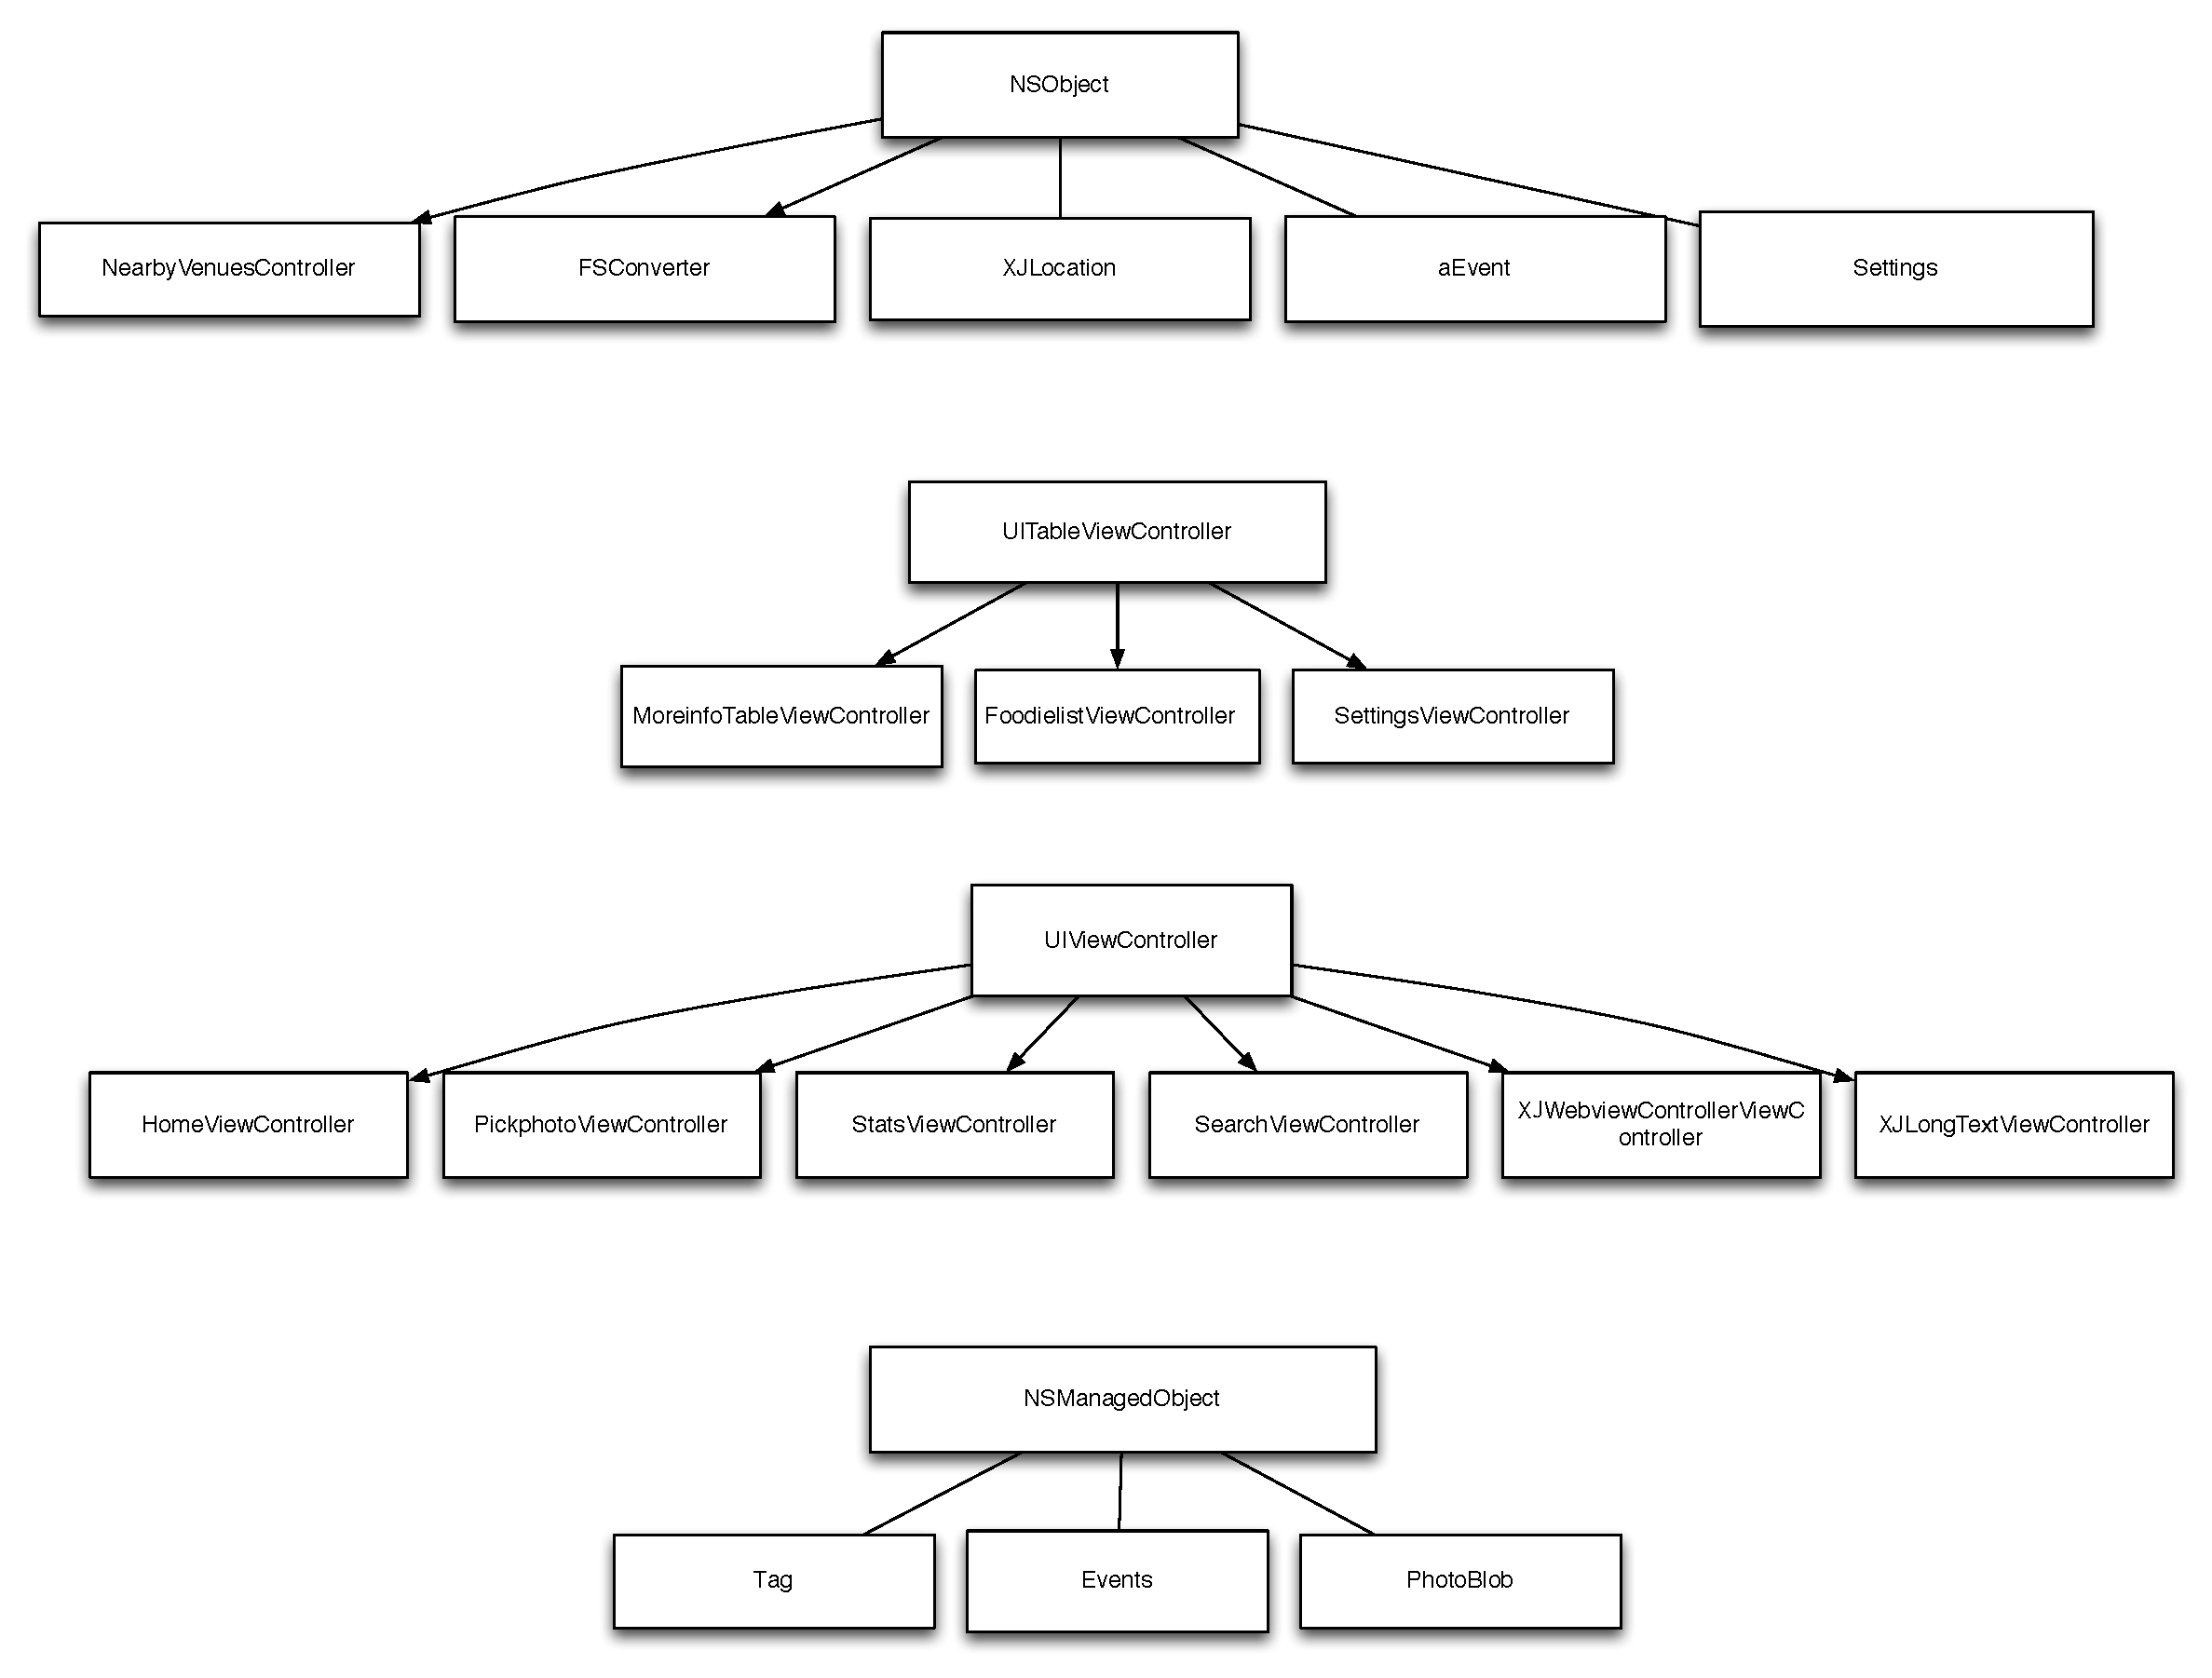
\includegraphics[%
    width=\figwidth, totalheight=\figheight, keepaspectratio]{./relationships.pdf}}
    \caption{Relationships with Cocoa Touch Framework}
	\label{fig:relationships}
\end{figure}
% subsection relationship_with_cocoa (end)
\subsection{Database Schema} % (fold)
\label{sub:database_schema}

	We used three tables for storing all the information from user. As Figure~\ref{fig:data-schema} shows, Events is the main table in the app. It provides fields ``address'', ``comment'', ``creationDate'', ``latitude'', ``longitude'', ``locationName'', ``rate'', ``thumbnail'', ``photoBlob'' and ``tags''. ``address'' field is used when user didn't find their ``locationName'' in location list which fetched from Foursquare API v2. ``Latitude'' and ``longitude'' is used for adding annotations in Map View. A 80*80 resolution thumbnail is stored for each event in order to accelerate loading food list table. \\ 
	
	``photoBlob'' has one to one relationship with ``photo'' in PhotoBlob table. Using a separate table should also help speeding up when we don't need to load photo while we still need to get the meta data of the event. \\
	
	Field ``tags'' has many to many relationship with ``photos'' in Tag table because one photo can labeled with many tags and one tag can relate to many photos.  
	

\begin{figure}
	\centering
    \SetFigLayout{1}{1}
    {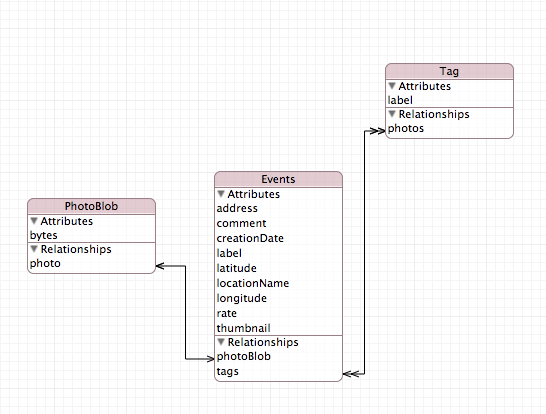
\includegraphics[%
    width=\figwidth, totalheight=\figheight, keepaspectratio]{./screenshots/database_schema.png}}
    \caption{Database Schema}
	\label{fig:data-schema}
\end{figure}

% subsection database_schema (end)

\subsection{Settings Property List} % (fold)
\label{sub:settings_list}

	When developing under iOS, we can also use another way to store the data we need. \emph{Property List} is used to store all information related to the app itself. For instance, using \emph{Property List} to store app display name, app version are commonly used in all apps for iPhone. \\
	
	``Fancy Foodie'' uses release number as main version string and git hash tag of the release as build string, so ``1.0 (build 3df55bb)'' is shown in Figure~\ref{fig:settings} which means that the main version number is 1.0 and build hash tag is 3df55bb. \\
	 
	 This app also use \emph{Property List} to store whether we need to save photo to album locally. If this option is enabled, the app will create an album  named ``Fancy Foodie Photos'' and put photos when creating the event in this album as shown in Figure~\ref{fig:album}.
% subsection settings_list (end)
% section software_architecture (end)



\section{Modules} % (fold)
\label{sec:modules}
Figure~\ref{fig:classdiagram} shows all the classes and public methods in the project. 

\begin{figure}
	\centering
    \SetFigLayout{1}{1}
    {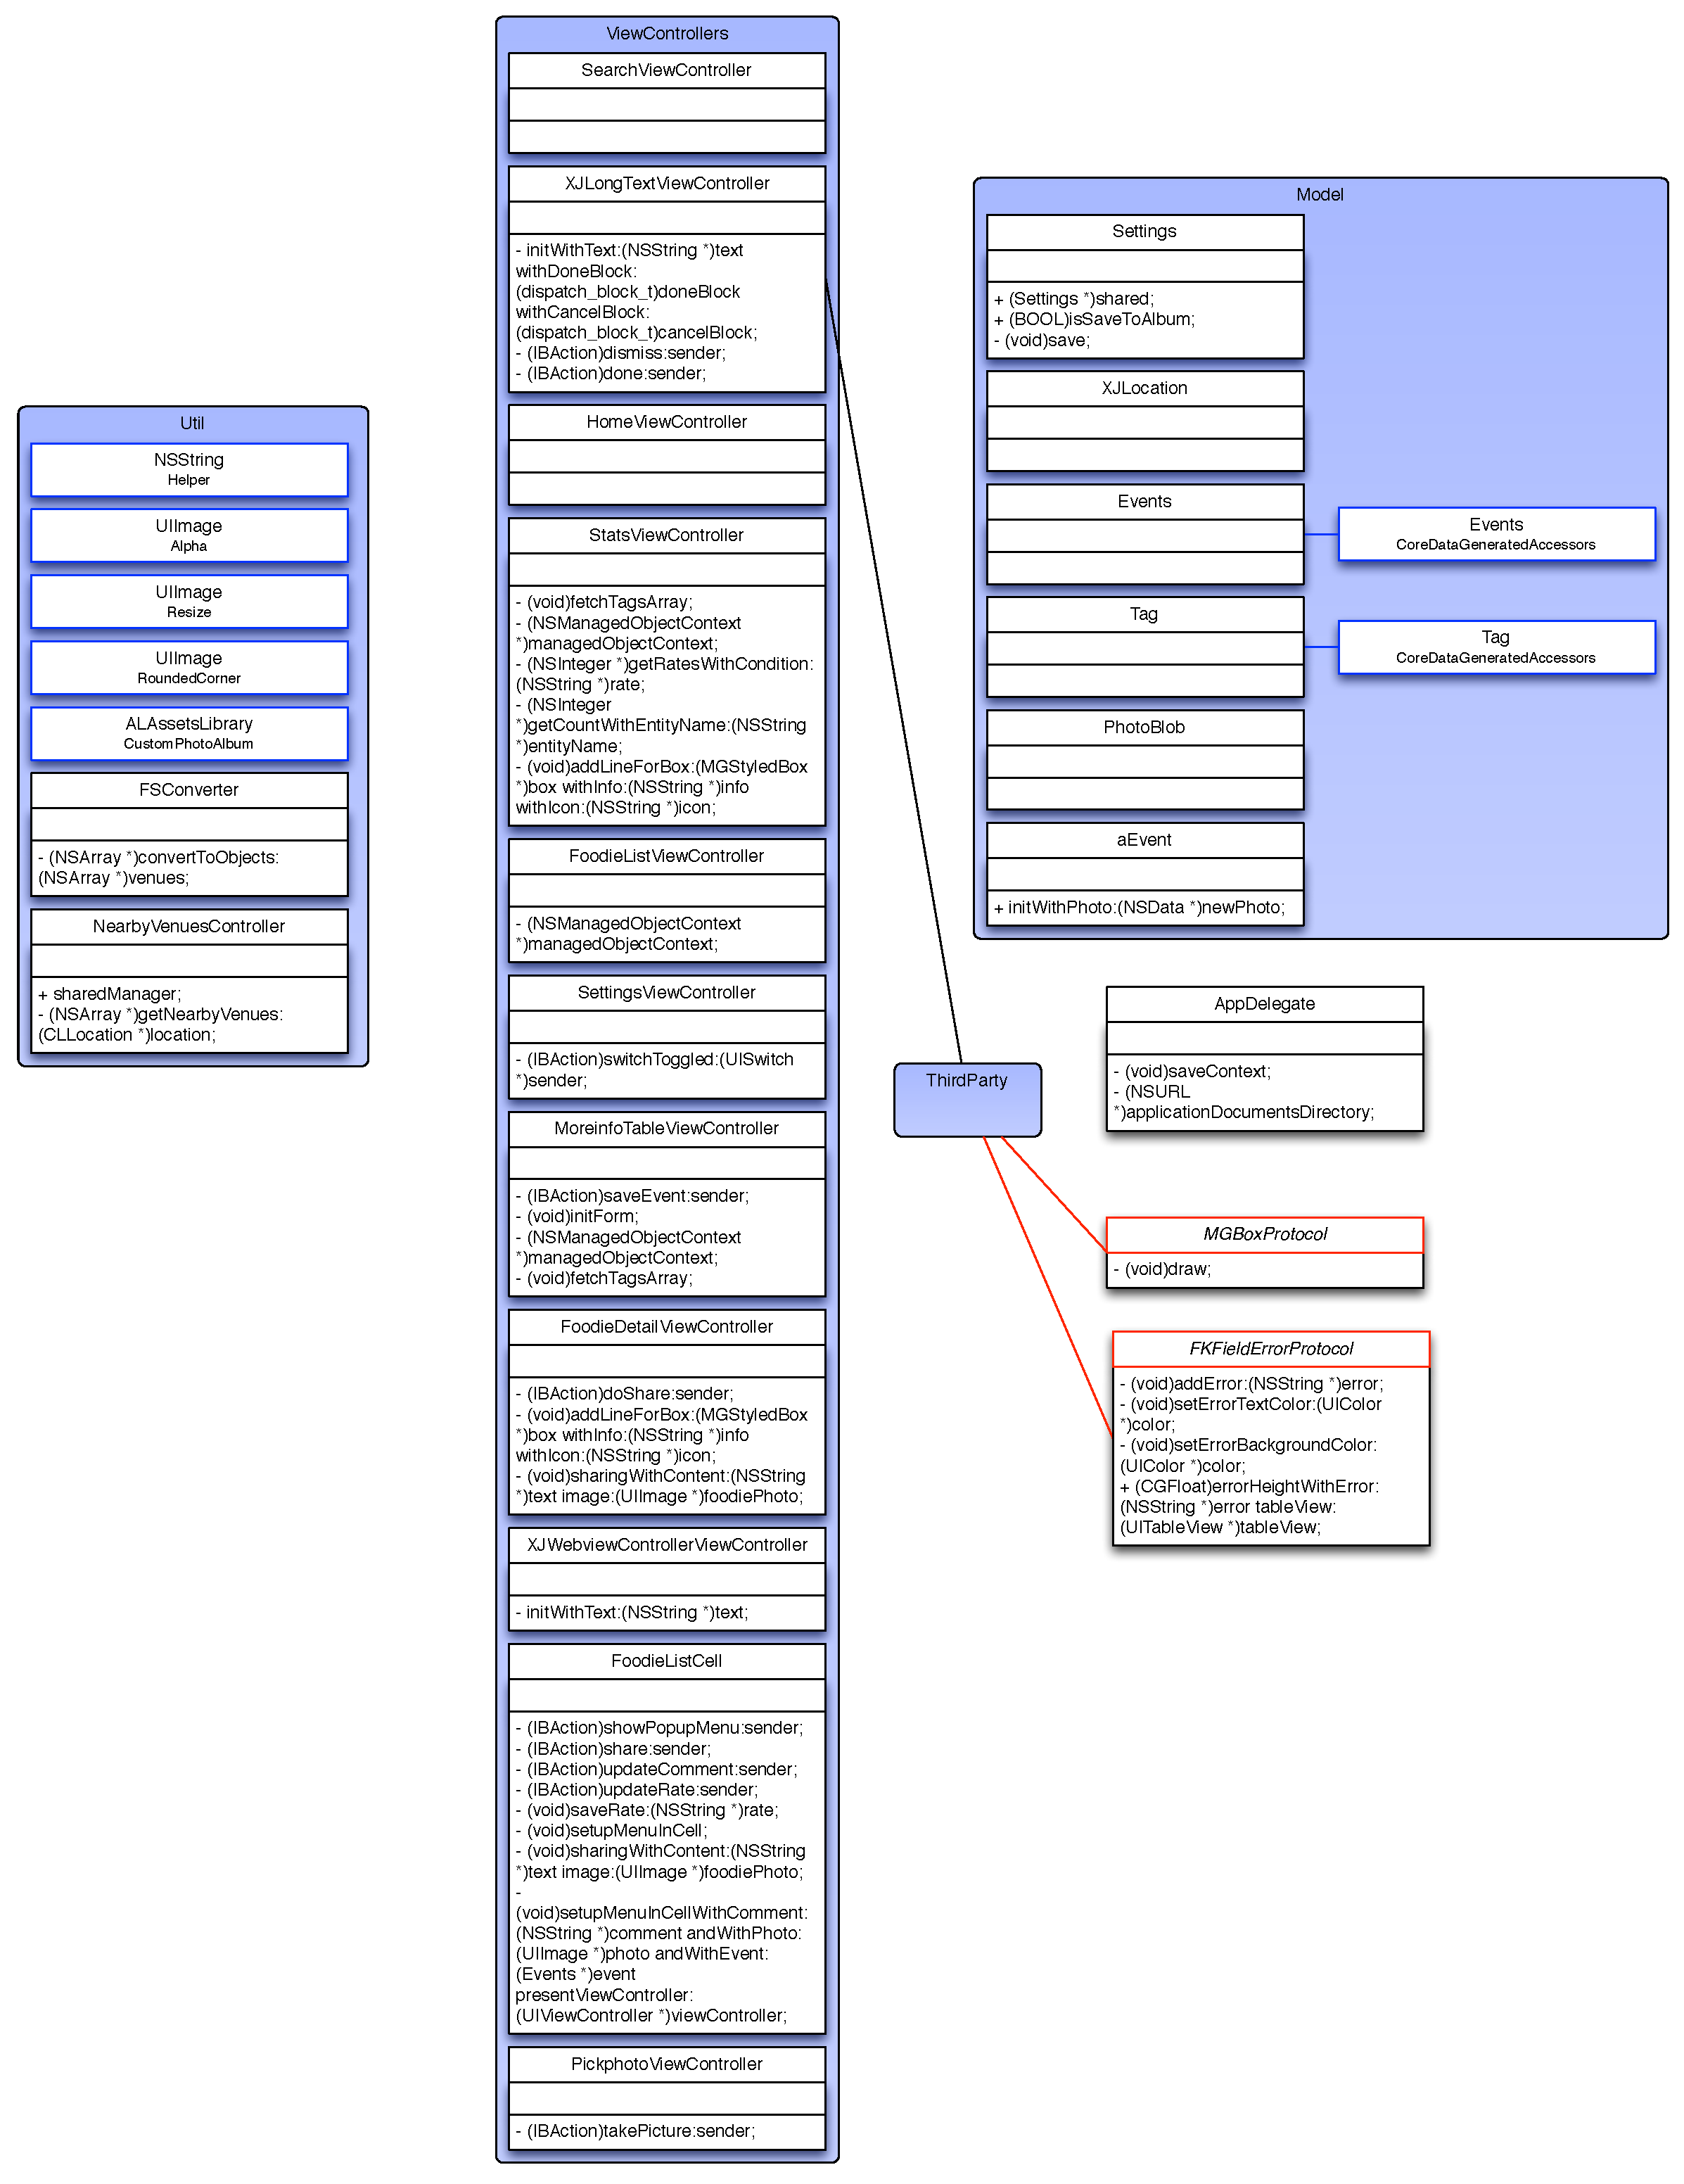
\includegraphics[%
    width=\figwidth, totalheight=\figheight, keepaspectratio]{./UML_Fancy.pdf}}
    \caption{Class-diagram of the project}
	\label{fig:classdiagram}
\end{figure}
% subsection overview_of_modules (end)

\subsection{View Controllers} % (fold)
\label{sub:view_controllers}
	Figure~\ref{fig:storyboard} shows main views in storyboard. In this project, we build it as a tab based application. Five tabs are created for different purposes. Home tab plays as a guide to create a food event; Food list tab shows all the events created before; Statistics tab shows all aggregated data; Searching tab is used to show all past events and searching by address to find the events; Setting tab is for configurations.
	
\begin{figure}
	\centering
    \SetFigLayout[5]{1}{1}
    {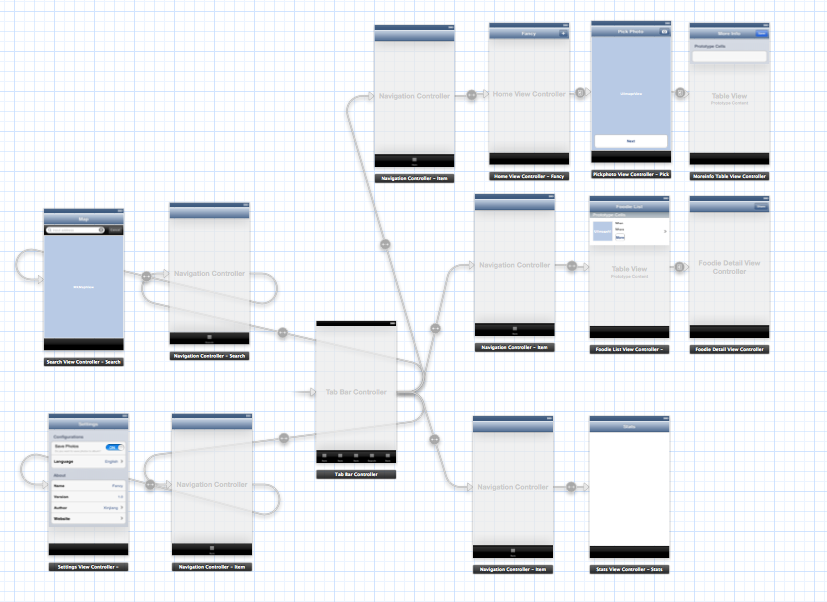
\includegraphics[%
    width=\figwidth, totalheight=\figheight, keepaspectratio]{./screenshots/storyboard-full.png}}
    \caption{Storyboard of Overview Fancy Foodie}
	\label{fig:storyboard}
\end{figure}

	The correspond viewControllers are list as follows.
	 
\begin{description}
	\item[HomeViewController] \ \hfill 
	Control views for users to start using the app.
	\item[PickphotoViewController] \ \hfill
	Present a preview of the photo chosen.
	\item[MoreinfoTableViewController] \ \hfill
	Control a form with all different types of information need to create a event.
	\item[FoodieListViewController] \ \hfill
	Display a table view to show all food events with thumbnail, relative date and location info. Control the logic of updating comments and rates.
	\item[XJLongTextViewController] \ \hfill
	Embedded a UITextView in UIViewController.
	\item[FoodieDetailViewController] \ \hfill
	Display all information of a particular event.
	\item[StatsViewController] \ \hfill
	Show statistics of all events.
	\item[SearchViewController] \ \hfill
	Provide a MKMapView, UISearchDisplayController and UITableView in this controller. 
	\item[SettingsViewController] \ \hfill
	Setting Options such as ``Save photo'',``language''. App name, version, author and support website are controlled here as well.
	\item[XJWebviewControllerViewController] \ \hfill
	Provide a UIViewController embedded with UIWebView.
\end{description}
% subsection view_controllers (end)

% subsection models (end)

\subsection{Third Party Libraries and Utility} % (fold)
\label{sub:third_party_and_utilities}
The following is a list of third party libraries used in the project.
		\begin{itemize}
		    \item TestFightSDK: Beta Testing on the fly.
		    \item BaseKit: Tools to create singleton class and better Location Manager.
			\item QBPopupMenu: Pop-up Menu User Interface
			\item CZPhotoPickerController: Preview of photos and better photo picker.
			\item FormKit: Form style tableview creation.
			\item BButton: Button with twitter bootstrap color schema.
			\item Foursquare2: Foursquare API version 2.
			\item MGBox: Table style boxes creation.
			\item SORelativeDateTranformer: Convert date to relative date such as ``One day ago''.
			\item FontAwesome: Adding icons to user interface.
			\item SVProgressHUD: Notification messages display.
		 \end{itemize}
A few important utility classes are listed as follows. 
		\begin{itemize}
		    \item NearbyVenuesController: Making request to Foursquare to get a list of locations nearby.
		    \item UIImage(Resize), UIImage(Alpha), UIImage(RoundedCorner): Tools to resize and modify images.
			\item ALAssetsLibrary(CustomPhotoAlbum): Saving images to custom album.
			\item FSConverter: Converting Foursquare feedback to an object.
			\item NSString(Helper): Providing convenient methods of NSString. 
		 \end{itemize}

% subsection third_party_and_utilities (end)
% section modules (end)

\section{Key Methods} % (fold)
\label{sec:main_methods}

\subsection{Insert New Event} % (fold)
\label{sub:insert_new_event}
	Figure~\ref{fig:storyboard-home} shows the procedure to add a new event. - (IBAction)saveEvent:(id)sender; in class MoreinfoTableViewController is called when a user finished editing all information in the form. First of all, we checked whether the save photo option is on or not. If it is on, we should save the image to an album named ``Fancy Foodie Photos''. Otherwise, go ahead and create an instance of Events called newEvent. Afterward, we assign all the information from user interface and save. Next step is to use the navigationController to pop to root view controller which is HomeViewController.

\begin{figure}
	\centering
    \SetFigLayout{1}{1}
    {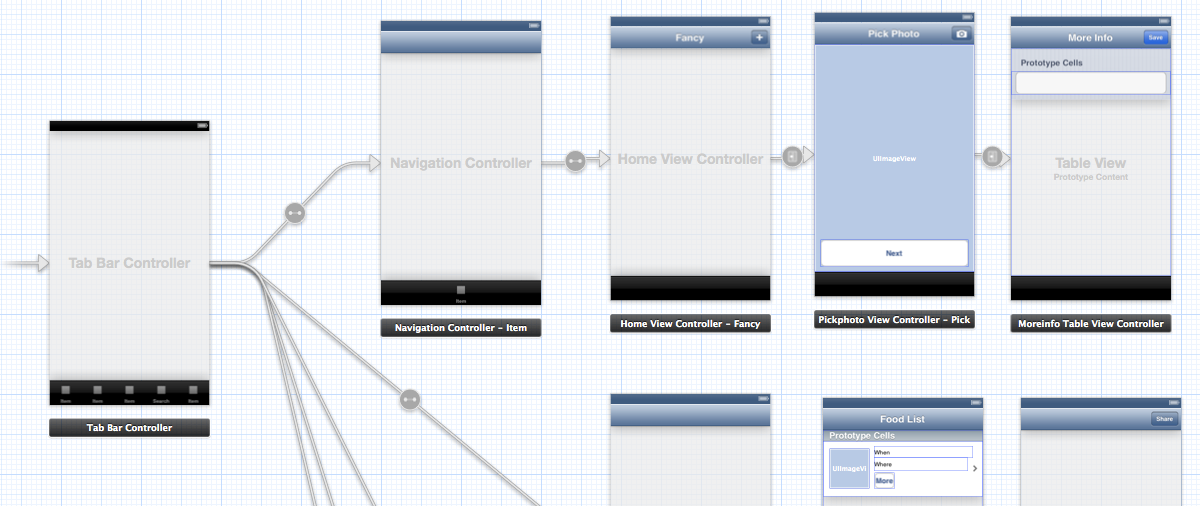
\includegraphics[%
    width=\figwidth, totalheight=\figheight, keepaspectratio]{./screenshots/storyboard-home.png}}
    \caption{Storyboard of Home Tab View}
	\label{fig:storyboard-home}
\end{figure}
% subsection insert_new_event (end)

\subsection{Update Event} % (fold)
\label{sub:update_event}

Updating event is actually updating rate or comment. When a user tapped on the pop up menu and chose comment option in Figure~\ref{fig:foodlist-menu}, - (IBAction)updateComment:(id)sender; in class FoodieListCell is called. Class XJLongTextViewController is used and presented as a modal (Figure~\ref{fig:foodlist-comment}). After typing in new comment and done button is tapped , it uses  NSManagedObjectContext to save the event and stored the updated data in the local database.

\begin{figure}
	\centering
    \SetFigLayout{1}{1}
    {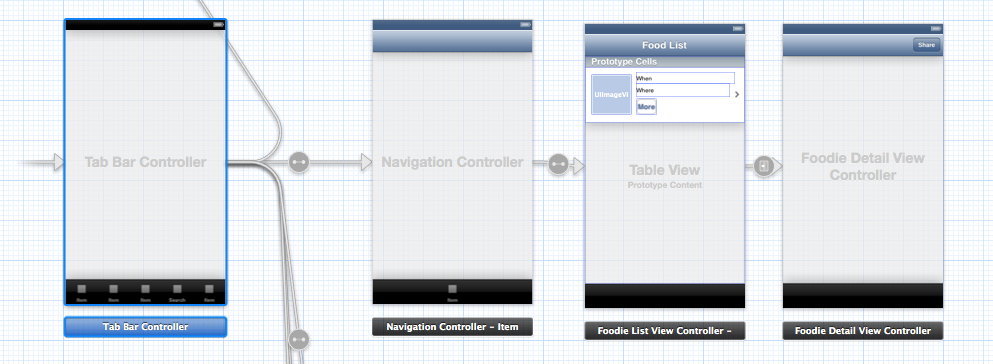
\includegraphics[%
    width=\figwidth, totalheight=\figheight, keepaspectratio]{./screenshots/storyboard-foodlist.png}}
    \caption{Storyboard of Food List Tab View}
	\label{fig:storyboard-foodlist}
\end{figure}

% subsection update_event (end)

\subsection{Delete Event} % (fold)
\label{sub:delete_event}

	Delete event is very simple in this app. In food list tab, you'll see a list of events. Swiping from right to left enable the delete button as shown in Figure~\ref{fig:foodlist-delete}.  After tapping on the button, - (void)tableView:(UITableView *)tableView commitEditingStyle:(UITableViewCellEditingStyle)editingStyle forRowAtIndexPath:(NSIndexPath *)indexPath; in class FoodieListViewController is called. In the method, it uses NSManagedObjectContext deleteObject to delete the event and save the result in local database after save function is called. Afterward, current tableview is refreshed as well.
% subsection delete_event (end)

\subsection{Searching Events} % (fold)
\label{sub:searching_logic}
	
	Searching events is done with MapKit API. All the events are fetched in during loading time. The events are annotated with red pins when the tab is loaded.   \\
	As shown in Figure~\ref{fig:map-address}, as the user is typing in the address, the searching string is passed to -(BOOL)searchDisplayController:(UISearchDisplayController *)controller
shouldReloadTableForSearchString:(NSString *)searchString; , so in that function, we're using CLGeocoder to guess the possible locations for that string. The possible locations are displayed in a table view. After the use choose one possible location, the central region will be focused on that area. At this time, the nearby events stored in database will appear in front of the user.
	

% section main_methods (end)
% chapter design (end)
\chapter{Testing} % (fold)
\label{cha:testing}

\section{Unit Test, Integration Test and System Test} % (fold)
\label{sec:unit_test_integration_test_and_system_test}
	
	All the modules are tested individually in separate Xcode project, and integrated into our main project \emph{Fancy Foodie}. After making sure the features are integrated with the main project, we build the project nightly, and test the function systematically with both stimulators and real cellphone which is iPhone 5.
% section unit_test_integration_test_and_system_test (end)

\section{Beta Testing} % (fold)
\label{sec:beta_testing}

	\emph{Fancy Foodie} use TestFlight to do beta testing on the fly. TestFlight provides a SDK for us to integrate it to the App. After integration, crash reporting will happen automatically. By logging in the dashboard of TestFlight, we could see all the information for each session of users as shown in Figure~\ref{fig:testflight-dashboard}.

\begin{figure}
	\centering
    \SetFigLayout{1}{1}
    {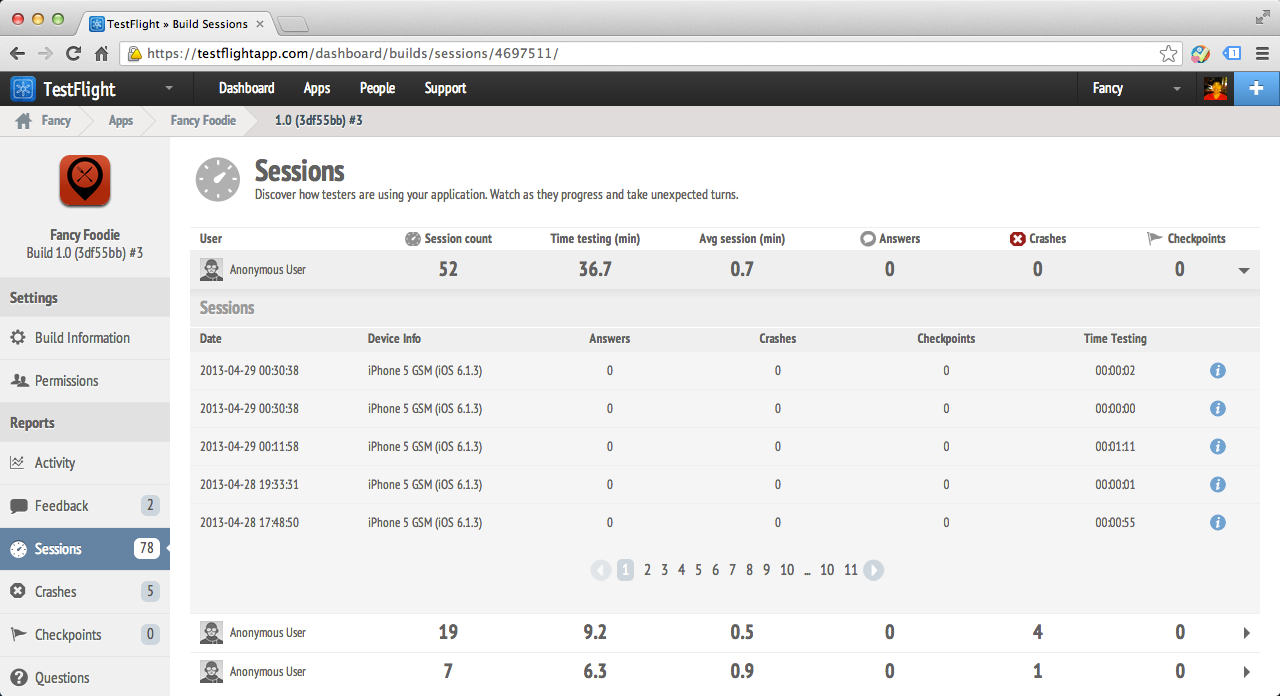
\includegraphics[%
    width=\figwidth, totalheight=\figheight, keepaspectratio]{./screenshots/testflight-dashboard.png}}
    \caption{TestFlight Dashboard}
	\label{fig:testflight-dashboard}
\end{figure}

% section beta_testing (end)

\section{iTunes} % (fold)
\label{sec:itunes}

	\emph{Fancy Foodie} is created in iTunes Connect on April 17, 2013. First submission was uploaded on April 17, 2013. But minor changes are made after that, so another submission was upload on April 23, 2013. Currently, \emph{Fancy Foodie} is waiting for review. After review, https://itunes.apple.com/us/app/fancy-foodie/id638036832?ls=1&mt=8 should be available to U.S. users. Anyone could download the App via that link.
% section itunes (end)

\section{Future Testing} % (fold)
\label{sec:future_testing}

Since it is ongoing project, future testing will be done by using TestFlight as well. We would set up checkpoint and create questionnaire to get better feedback from users. 
% section future_testing (end)
% chapter testing (end)
%\chapter{Future Work}

Yelp Intergation 

Centeral Database

Multi-languages

beta Test


\chapter{Conclusion}

This project is successfully finished in time with good functionalities overall. It could provide users to take picture of food they like and create tags, location information, rates, and comments to the food. At the time, it provides convenient methods for users to share those food with their friend by social media such as Facebook, Twitter, Weibo etc.. A map view and statistics view are created for users to have better understanding of their preferences. \\

There are still more features could be done in future. Since Yelp is a good resource of restaurant information, the app could pull more information from Yelp in order to give users more about the place they eat at. A central database is needed to making users communicate with each other such as making comments to friends food inside of the app. Chinese is my mother tongue, so I'm hoping to adding multi-language feature for the App. In this way, more people could be able to use the App. Last but not least, a larger pool of testers should be included in beta testing process.

\clearpage
\addcontentsline{toc}{chapter}{Acknowledgements}
\chapter*{Acknowledgments}
\vspace{1.0in}

I would like to thank open source community. Without them, I probably need much more time to finish this project. \\

I would also like to thank Jakob Eriksson and Ugo Buy. Prof. Eriksson gave me a lot of valuable suggestion for my project.  Prof. Buy also provided helpful suggestion on the report. Both Prof. Eriksson and Prof. Buy give a good evaluation of my work. \\

Special thanks to all my friends who made tremendous comments about my app and all my colleagues in EXACT Sports LLC who slow me down in the right way so that I can make the project better. \\

%{Xinjiang Shao}\\ 
\leavevmode
\\
\\
\\
\\
\\
Xinjiang Shao \\
{April 2013}\\
{University of Illinois at Chicago}\\
\newpage

\addcontentsline{toc}{chapter}{References}
\begin{thebibliography}{99}

\bibitem{citation-1-name-here}<Name of the reference here>,\ \url{<url here>}

\bibitem{citation-2-name-here}<Name of the reference here>,\ \url{<url here>}

\end{thebibliography}


\end{document}
